\documentclass{CSEThesis}
% Standard packages
\usepackage{amsmath}        % Extra math definitions
\usepackage{graphics}       % PostScript figures
\usepackage{setspace}       % 1.5 spacing
%\usepackage{psfig,epsfig}
\usepackage{multicol}
\usepackage{subcaption}
\usepackage{hyperref}
\usepackage{epsfig,color}
\usepackage{tcolorbox}
\usepackage{minted}
% \usepackage[superscript, biblabel, nomove]{cite}
% Custom packages
%\usepackage[first]{datestamp}   % Datestamp on first page of each chapter


\usepackage{color}
%===== page layout
% Define the side margins for a right-side page
%\insidemargin = 1.3in \outsidemargin = 0.9in
% Above margin is space above the header
% Below margin is space below footer
%\abovemargin = 1.5in \belowmargin = 0.05in


\newcommand{\git}{https://github.com/sourabh2311/btp/blob/master/Compiler/}
\newcommand{\iph}[2]{
   \includegraphics[width=#1\textwidth,height=#1\textheight,keepaspectratio]{#2}
}
\newcommand{\ph}[1]{
   \includegraphics[width=0.5\textwidth,height=0.5\textheight,keepaspectratio]{#1}
}
\newcommand{\tfbox}[1]{
\begin{tcolorbox}[colframe=purple!75!black,title=Associated File(s) Link]
#1

\textit{Please see comments in the file(s) for more details.}
\end{tcolorbox}
}

\newcommand{\nbox}[1]{
\begin{tcolorbox}[colframe=purple!75!black,title=Note]
#1

\end{tcolorbox}
}
\newcommand{\ghref}[1]{
   \href{\git #1}{#1}
}

\btptitle = {Tiger to RISC V Compiler} % { and } are needed around your name
\name = {Sourabh Aggarwal}          % and other feilds. don't remove.
\rollno = {111601025}
\email = {111601025@smail.iitpkd.ac.in}
\guide = {Dr. Piyush P. Kurur}

\setminted{breaklines=true, tabsize=2, breaksymbolleft=}

\begin{document}

\begin{titlepage}
	\begin{center}
		\textheight 15.5in \textwidth 12.5in {\large\sf  \textbf{\the\btptitle}}\\[12ex]
		{\small{\textsl{ \textbf{A Project Report Submitted \\
		in Partial Fulfillment of the Requirements \\
		for the Degree of \\
		[3ex]\small \bf Bachelor of Technology}}}}\\
		[16ex] \emph{by}
		\\[2ex]
		{\sf \sf \textbf{\the\name}\\
		(\the\rollno)}\\[1ex]
		\emph{under the guidance of}\\[2ex]
		{\sf \bf \the\guide} \\[7ex]

		\vspace{1.2in}

		\begin{figure}[!h]
			\centering
			
\includegraphics[width=0.15\textwidth]{IITPkdFullLogoColor}
		\end{figure}



		{\small\bf DEPARTMENT OF COMPUTER SCIENCE AND ENGINEERING}  \\[1ex]
		%{\small \bf{INDIAN INSTITUTE OF TECHNOLOGY PALAKKAD}}
		%\\[2ex]
		%
		%  {\color{red} \hrule height 0.5ex}
		% \vskip 1ex
		% May \the\year 
	\end{center}
\end{titlepage}



\raggedbottom
\doublespacing
\pagenumbering{roman}
\chapter*{\centering \underline{CERTIFICATE}}
\vskip 2ex \emph{\quad This is to certify that the work contained
in this thesis entitled ``\textbf{\the\btptitle}'' 
is a bonafide work of \textbf{\the\name}
(\textbf{Roll No. \the\rollno}), carried out in the Department of
Computer Science and Engineering, Indian Institute of Technology
Palakkad under my supervision and that it has not been submitted
elsewhere for a degree.} \vskip 15ex

\begin{flushright}
	\textbf{Dr. Piyush P. Kurur}\\
	Associate Professor \\
	Department of Computer Science \& Engineering \\
	Indian Institute of Technology Palakkad
\end{flushright}
\hfill 
\hfill 






\chapter*{\centering Acknowledgements}
\quad Write acknowledgements, if your want to.



\tableofcontents 

\cleardoublepage
\phantomsection
\addcontentsline{toc}{chapter}{List of Figures} 
\listoffigures 

% \cleardoublepage
% \phantomsection
% \addcontentsline{toc}{chapter}{List of Tables} 
% \listoftables

\pagenumbering{arabic}
\def\headrulehook{\color{black}}      % Color the header rule

%========== Chapters
\typeout{}
\chapter{Introduction}

This project aims to write a compiler to compiler Tiger to RISC V assembly code.

\nbox{Before proceeding it is important to read about Tiger language from \cite{tigerbook} \textit{(read Tiger Reference Manual in Appendix)}.}

Beyond the specification of the language mentioned within text \cite{tigerbook}, my Tiger specification includes abstractly two more things:-

\begin{enumerate}
	\item Real number support.
	\item Objective functionality support.
\end{enumerate}

Real numbers enjoy first class support just like integers, strings and can be used exactly as integers.

\section{Grammar Additions}

$exp \rightarrow$ \textit{real-literal}

$\rightarrow$ \textit{\textbf{new} class-id}

$\rightarrow$ \textit{lvalue.id()}

$\rightarrow$ \textit{lvalue.id(exp\{, exp\})}

\textit{dec} $\rightarrow$ \textit{classdec}

\textit{classdec} $\rightarrow$ \textit{\textbf{class} class-id \textbf{extends} class-ids \{\{classfield\}\}}

\textit{class-ids} $\rightarrow$ \textit{id\{, id\}}

\textit{classfield} $\rightarrow$ \textit{vardec}

\textit{classfield} $\rightarrow$ \textit{fundecs}

\section{Specifications For Objective Tiger}

For the purpose of understanding the below points, refer \ref{fig:wmi}

\begin{figure}
	\centering
	\iph{0.80}{assets/lastphase/TigerObjectWithoutMI2-min.png}
	\caption{Classes Demo I}
	\label{fig:wmi}
\end{figure}

\begin{itemize}
	\item To simplify implementation, all declared \textit{classes} (irrespective of being in different environment) should have unique name.
	\item \textit{vardec}, \textit{fundecs} could be \textit{overridden} by the subclass but the types should be preserved as it has to be backward compatible.
	\item \textit{vardec}'s within the class shall not use this subclass fields for its initialisation as there is no self to fetch them.
	\item As evident from grammar specification, there is no "method" but our usual "functions" and thus mutually recursive methods are supported.
	\item Type casting of a subclass to its superclass is supported both in variable assignment and as in function argument. This is termed as "SUPERTYPE". We can see in line 19 that though variable \texttt{c} is of type \texttt{Car} yet we have assigned it to a variable of type \texttt{Vehicle}. Similarly in line 24, when executing \texttt{c.await(t)}, we can very well see that the \texttt{await} function expects an object of type \texttt{Vehicle} but we have given an object which is a subclass of it.
	\item There is also a support to check whether an object 'x' is of its original class 'X' or any of the superclass of 'X' via \textit{ISTYPE(objectName, ClassName)}. \textit{ClassName} is to be given as a \textit{string} whereas the other parameter shall be \textit{var}.
	\item Multiple inheritance is supported but the classes to be extend should be \textit{disjoint} and thus should have no field in common.
	\item Classes to support solely \textit{vars} and \textit{fundecs} which \textit{could} be redefined as evident by redefinition of variable \texttt{position} and function \texttt{move} in line 14, 15 respectively.
	\item Concept of \textit{self}. When calling a function of an object, one need not pass its own discriptor which is done via compiler but when declaring the function of a class, one needs to mention \textit{self} as an argument.
\end{itemize}


\section{Compile Time Arguments}

Since there are so many choices offered to a user when using this compiler. For instance:-

\begin{enumerate}
	\item Option to give filename to print IR Tree at. Flag = \texttt{ir}. Default = \texttt{TextIO.stdOut}.
	\item Option to give filename to print instructions before register allocation at. Flag = \texttt{ba}. Default = \texttt{TextIO.stdOut}.
	\item Option to choose which string algorithm to be used for displaying suggestions in case of mistyped word. Flag = \texttt{sa}. Default = \texttt{0} (i.e. Levenshtein algorithm).
\end{enumerate}

I have implemented feature for users to give compile time flags. Note: I mention "flags", thus user has an option to not define it, in which case default flag will be taken. See \ref{fig:flags} for an example usage.


\begin{figure}
	\centering
	\iph{1}{assets/flags-min.png}
	\caption{Compile time arguments}
	\label{fig:flags}
\end{figure}

\section{How To Compile?}

One needs to first \textit{make} the files visible in \textit{sources.cm} as \texttt{CM.make ("sources.cm")} then simply compile the file using the command (in sml), \texttt{Main.compile(FilePath, Arguments)}. For an example please see the above subsection and aswell the file \texttt{fileTest.sh}, contents of which are listed in \ref{fig:sm}.

One can now run the compiled RISC V code using \href{https://github.com/TheThirdOne/rars}{RARS} like \texttt{java -jar rars1\_3\_1.jar sm nc TestFiles/filename.tig.s}

\section{Organisation of Report}

The second chapter explains how to add Objective functionality to Tiger. Third, Fourth chapter briefly explains the work done for this project, i.e. $8^{th}$ Semester and $7^{th}$ Semester respectively.

These chapters also explains various functionalities provided by my Compiler. The code written for this compiler is enormous and the remaining part of the report gives documentation on each of these files in an understandable order.
\cleardoublepage
\typeout{}
\chapter{Adding Objective Support in Tiger}

As explained in first Chapter, Classes can have only two type of fields, viz., \textit{vars} and \textit{functions}.

\section{Support for \textit{vars}}

One can understand on how to add support for \textit{vars} provided one understands the working of \textit{record}. Abstractly one can think of Class as being union of \textit{vars} and \textit{functions}. Thus, these two could be \textit{separately} supported. If we forget about \textit{functions} then the Class (besides other Class functionalities like Multiple Inheritance, "SUPERTYPE", etc) simply reduces to a \textit{record}. So \textit{vars} support has been added as its done in case of \textit{records}. Please see \texttt{semant.sml} for more details.

\section{Support for \textit{functions/methods}}

Unlike \textit{vars}, which could be "stored", \textit{functions} are "declared". One should understand this as this is pivotal to successfully implement \textit{functions}. Thus, if we are adding Class type to our environment, we shall add its declared \textit{functions} in our environment with \textit{certain} modification. This modification is needed as these functions are not "outside" Class's declaration thus can't be called upon without corresponding Object. One way to achieve this is to mask the functions name (say "F") of Class (say "C") to "Class\_C\_F". This is how I handle the functions.

\section{Supporting Single Inheritance}

\begin{figure}
	\centering
	\iph{0.50}{../sem8_presentation2/singleInheritance.png}
	\caption{Single Inheritance Program}
	\label{fig:SI1}
\end{figure}

\begin{figure}
	\centering
	\iph{0.50}{../sem8_presentation2/SIV.png}
	\caption{Single Inheritance Fields Allocation}
	\label{fig:SI2}
\end{figure}

Since we must support backward compatibility, the idea of "SUPERTYPE". Superclass's fields should be listed before the Subclass's fields as shown in figure \ref{fig:SI2} of program \ref{fig:SI1}. Since I support for fields redefinition, one should be cautious when implementing this.

\section{Support for Multiple Inheritance}

This would have been easy in case we were to not support "SUPERTYPE". It is the combination of Multiple Inheritance and backward compatibility that makes this problem tough.

To understand this, see \ref{fig:MI1} and \ref{fig:MI2}. We can see that we just can't list the fields linearly for any class and inevitably there are gaps left.

\begin{figure}
	\centering
	\iph{0.50}{../sem8_presentation2/MI.png}
	\caption{Multiple Inheritance Program}
	\label{fig:MI1}
\end{figure}

\begin{figure}
	\centering
	\iph{0.50}{../sem8_presentation2/MI2.png}
	\caption{Multiple Inheritance Fields Allocation}
	\label{fig:MI2}
\end{figure}

\begin{figure}
	\centering
	\iph{0.50}{../sem8_presentation2/MI3.png}
	\caption{UFDS Example}
	\label{fig:MI3}
\end{figure}

To handle this, we can "statically" analyse the complete program and reduce this problem to graph coloring. Idea is to add an edge between \textit{vars} which could possibly end being in the same class. Then we would be ended with disjoint Cliques which could then be colored.

But we can do better. As the graph is simply disjoint cliques, each node in a component would receive different color. Thus we can simply use UFDS data structure and color each element of the set with different color. Here we just need to join the set containing \textit{vars} of Superclasses with Subclass. See \ref{fig:MI3} for an example for the code \ref{fig:MI1}.

\section{Support for \textit{ISTYPE}}

With this section, I will also explain on how to support type casting. Basically for type casting we just need to check whether this type is even compatible with given type which would be possible if the Class concerned is Superclass or original class of the given object. So for given class, one should store the list of all classes which it extends. Now to see type casting or type compatibility, we try to match the given class with the classes in this list and continue recursively until we reach the base Object Class.

Now \textit{ISTYPE} uses this procedure to check validity. This is done in \texttt{semant.sml} and after determining, I here itself replace this program code with simply its answer which is either integer 0 or 1.
\cleardoublepage
\typeout{}
\chapter{What Has Been Achieved This Semester}

\section{Miscellaneous Improvements}

\subsection{More Graceful Error Termination}

Earlier in lexical phase, as soon as an error was found, I was raising an exception but it could be better presented as simply an exit failure, or even better an exit success with just my simple lexer error. Which reduces the error output received by the user. Figure \ref{fig:gr1} and \ref{fig:gr2} shows the reduction in those "uncaught..." lines.

\begin{figure}
	\centering
	\iph{0.80}{assets/lexError-min.png}
	\caption{Graceful error termination - before}
	\label{fig:gr1}
\end{figure}
\begin{figure}
	\centering
	\iph{0.80}{assets/lexError3-min.png}
	\caption{Graceful error termination - after}
	\label{fig:gr2}
\end{figure}

\subsection{Simplified "Make" Process}

Earlier, the bash script to compile the given file required to concatenate the output with the \texttt{runtime.s}. Now it has been significantly simplified and the compilation process is reduced to just \texttt{Main.compile filename (optional flags)}. This concatenation business is now handled in the \texttt{Main} file itself. See \ref{fig:sm}.

\begin{figure}
	\centering
	\iph{0.80}{assets/makeS-min.png}
	\caption{Simplified Make}
	\label{fig:sm}
\end{figure}

\subsection{Drew My Own Tiger}

Just for fun, I drew my own Tiger logo. See \ref{fig:tig}.

\begin{figure}
	\centering
	\iph{0.80}{assets/tiger-min.png}
	\caption{Tiger Logo}
	\label{fig:tig}
\end{figure}

\subsection{Printing IR Tree As Well As Generated Code Before Register Allocation}

The author of the book gives the program to achieve this. But due to changes commited by me in IR Tree, etc. hindered myself from using that code as now it would demand modifications to use but I didn't find much use of it later. Now as I was getting stuck time and again in various phases of these new improvements I was targeting. It became necessary to study IR tree and the code before register allocation to pin point where exactly the error is. See \ref{fig:ir} and \ref{fig:ba}.

\begin{figure}
	\centering
	\iph{0.80}{assets/ir-min.png}
	\caption{IR Tree}
	\label{fig:ir}
\end{figure}


\begin{figure}
	\centering
	\iph{0.80}{assets/ba-min.png}
	\caption{Code before register allocation}
	\label{fig:ba}
\end{figure}

\subsection{Others}

\begin{itemize}
	\item Added more details in the project’s documentation (with more diagrams) to make it more useful for lucid revision. Along with general improvements in code.
	\item Removed External Calls (this lead to simplification in code generator, semantic, translate and risc frame files).
	\item \texttt{FP} is indispensable, thus I decided not to remove it by calculating it using \texttt{SP}.
\end{itemize}

\section{Simplified String Comparisons}

Comparing strings in  a program is indispensable. Therefore, it is inconvinient to have user type a function each time there is a need to call a string function. Thus, I have added this funcionality where string comparisons can be done naturally.

\textbf{Idea} behind its implementation is that whenever lexer sees \texttt{str1 > str2}. Then in semantic analysis phase, we should determine whether both sides of an operator are of type strings or not. If that is the case then we can delete this node and replace it with a function call as inequalities are like conditions. So one should have supporting functions defined in \texttt{runtime.s} along at other places. See \ref{fig:sc} for an example usage.

\begin{figure}
	\centering
	\iph{0.80}{assets/stringC-min.png}
	\caption{String Comparisons}
	\label{fig:sc}
\end{figure}

\section{Suggestions for Mistyped Words}

Tiger's target has always been to continue in case there are any mistakes and show maximum possible mistakes to the user at once.

Keeping this aim in mind, it is as well desired to print suggestions for a mistyped word which could be either a variable/function or a type name.

Earlier I abstracted out \texttt{Not Found} errors in semantic phase but failed to proceed from that point in that semester. This semester, I began on continuing from where I left. I did \textbf{huge} amount of changes where I completely removed \texttt{symbol.sml}, \texttt{table.sig} and \texttt{table.sml}. I replaced their used everywhere with \texttt{atom}. And as this was a huge change, I expected many errors. Ultimately I lost to the errors and as I got the new insights, this was anyway not needed. \textbf{Idea} is that, anytime if somebody calls this symbol function, we are storing this new symbol. So if one is anyway storing a symbol, better I can just query this \texttt{symbol.sml} to ask whether a string is present in symbol table or not. If it is present I can get a corresponding symbol which I can use to check whether that symbol is present in a given environment. I can even map an integer (denoting string's length) to a set of symbols. Keeping these things in mind, I have implemented two algorithms:-

\subsection{Algorithm I}

In this algorithm, I am using a map, which maps an integer (denoting string's length) to a set of symbols. Now each time, I encounter a "Not Found" error, I get from this map, sets having strings of length 0 or unit distance away from the given string. Now we can use \textbf{Levenshtein's} algorithm to check for minimum edit distance of the given string from this set. Time complexity will work out to be: $\mathcal{O}(m * l^2 * log^2(s))$. Where $m$ equals strings in this set, $l = max(|strings|)$ and $s$ equals total symbols in the environment, we have this log factor for this look up and as well as lookup to get sets corresponding to that length, and quadratic factor for minimum edit distance DP algorithm.

\subsection{Algorithm II}

This is comparatively quick algorithm which successfully attempts to find string which are unit distance apart. The idea is that we can easily find a symbol corresponding to a string (if such a symbol exists) from our \texttt{symbols.sml} in $log$ factor, then, we can simply check whether this symbol exists in our environment in another $log$ factor. Now a string can be unit distance apart by a character deletion, or insertion or replacement (I as well implemented swap check function which is very common form of error). Trying all these possibilites, time complexity works out to be: $\mathcal{O}(log(s) * l * |\Sigma|)$ where $s$ is as defined before, $l$ equals length of the given string and $\Sigma$ equals set of characters which are to be tried for replacement (this although can be treated as a constant and removed from this asymptotics).

Both the algorithms can have their advantage for certain test cases, it is left to the user which algorithm to use with the help of the flag \texttt{sa} as mentioned before. Algorithm 1 is better when there are less number of symbols and user is interested in just the minimum possible edit distance away string which needn't be just one character away.

Implementation of these algorithms can be found in \texttt{symbol.sml}.

\section{Real (Float) Implementation - Phase I}

Implementing real number support is a huge challenge as it requires A-Z modifications and in this 4000+ lines of code, even one bug could be fatal and difficult to detect thus making it important to identify at which phase is the error coming. Is it coming in IR generation phase or Code generation phase. Keeping this in view, I augmented \texttt{printtree.sml} file given by the author to streamline it with the modifications in my IR tree. There were lots of changes required which I will mention in the phase II of this.

Reals have dual behavior. They behave partly as strings and partly as integers. One cannot simply load a floating point register as in case of integers like \texttt{li a1, someInteger}. They need to be first declared at top in \texttt{.data} field just like strings, then their address loaded again just like strings, then finally they have to be loaded to a floating point register in a different manner like \texttt{flw fa1, address}.

In Tiger specification, each time a function returns a value, it is expected to return an integer value. Similarly, everywhere it is assumed that \texttt{temp} will be assigned an integer value. Changing nature of \texttt{temps} and full fledged support of reals would imply change at almost all files, which is cumbersome. One can get away from this by treating floats like strings, ofcourse one would require to make changes in all the phases before code generation with dedicated type for floats but treating floats just like strings, would mean that we would always have to play with just address which is an integer and not with any real value as such. One can levy the pain to pre defined functions for performing arithmetic and comparison operations with the drawback that they will return result, just like in case of strings, an address of a newly allocated memory. This is the only drawback of this as one mainly tries to avoid memory accesses. This phase however implements this as it forms a basis for phase II in which I provide complete support for floats.

This phase in itself as well demanded lots of modifications which was not easy. All the extra functions written in \texttt{runtime.s} were removed in phase II.

Example of changes required in this phase are given in figure \ref{fig:rphi1} and \ref{fig:rphi2}.

\begin{figure}
	\centering
	\iph{0.80}{assets/rphi1-min.png}
	\caption{Real I Implementation Glimpse (a)}
	\label{fig:rphi1}
\end{figure}

\begin{figure}
	\centering
	\iph{0.80}{assets/rphi2-min.png}
	\caption{Real I Implementation Glimpse (b)}
	\label{fig:rphi2}
\end{figure}

\section{Register Allocator}

My last sem's compiler's register allocator was incomplete and a crude implementation of the algorithm given in the text. It was without coalescing which is essential to minimize the spills and different register's use (in move instruction). The book has a whole chapter dedicated to this subject. It takes time to read and understand this algorithm, so it took me some days to finally appreciate this algorithm. While implementing this algorithm, for purpose of optimizations, I did modifications among other files as well list using set everywhere from which one can easily add / delete an entry.

The algorithm given in the book is huge and requires careful implementation. After the algorithm's implementation there were major issues I was facing due to some errors. Each morning, I could get an insight on a potential bug.

To identify bugs, one require critical scrutiny of the generated assembly code. One need's to generate small examples which break the code, i.e. deviate from expected behavior. After careful examination of one such program, I realised that \texttt{ra} register isn't getting backed up. And after \textbf{circling} through many places, I found the error was at incorrectly setting up \texttt{dst} registers when calling a function, here I missed to include \texttt{ra} register due to which it wasn't causing an interference with its use. See \ref{fig:eb}.

\begin{figure}
	\centering
	\iph{0.80}{assets/mistake1-min.png}
	\caption{Bug in Register Allocator}
	\label{fig:eb}
\end{figure}

I have taken this example to highlight, how a little bit of mistake could be the cause of stress and so much of time.

Juggling through these errors (like one of my major error was that I had been inserting in stack in reverse direction), I came to a point where I felt stuck, I was loosing hope each passing moment and felt that I finally have to give up on this, on so much of changes that I have done. The issue was with the algorithm presented by the author where he missed very important line. Refer \ref{fig:culprit} where you can see that checking whether \texttt{v} is in the precolored nodes or not was critical as precolored nodes should not be touched.

\begin{figure}
	\centering
	\iph{0.80}{assets/culprit-min.png}
	\caption{Critical Error in Book's Algorithm}
	\label{fig:culprit}
\end{figure}

This was a real relief and a mark of something really innovative done in this project. Final generated code was significantly lower than earlier, demonstrating the power of coalescing.

\section{Real (Float) Implementation - Phase II}

As remarked, this phase attempted to provide full fledged real numbers support. I did huge number of modifications as:-

\begin{enumerate}
	\item Everywhere when doing \texttt{T.newtemp} one need to \textbf{specify} whether, real or an integer register is needed.
	\item To provide this information, in places one needs to know that whether called function arguments are real or not. And also whether a function returns a real value or not.
	      \begin{enumerate}
		      \item This sparked changes in \texttt{riscframe.sml}, \texttt{semant.sml}, \texttt{translate.sml}, \texttt{tree.sml} and many other files.
		      \item Even in canonisation phase, one needs to generate a new temporary for shifting function's return value, thus for this reason as well one need IR tree to contain information about functions return value.
	      \end{enumerate}
	\item Assign statement needed to know whether parameters are real or not as then only one can do \texttt{RMOVE} or an integer move, \texttt{MOVE}. This is needed as floating points are moved differently.
	\item Similarly floating points are loaded and stored using different instructions than integer, this demanded for addition of \texttt{RMEM}.
	\item Code generation was thus heavily modified as it needed to generate correct code for all these changes. This requires a great amount of thinking as same things can be obtained using different means and one should try to do least changes in IR tree.
	\item The way code was generated when calling a function was as well heavily modified as one needs to differentiate a real and non real value as their moves, memory access is different. In that case also one needs to identify whether an access is in register or memory.
	\item New frame generation in \texttt{riscframe.sml} was heavily modified as now shift instructions needed to take care for both ints and real temporaries and also access had to specifically generated according to argument type.
	\item All in all there were heavy changes in almost all the files including the changes which were done previously as now reals can not be treated simply like strings, thus their basic expression had to be changed and this change has to be thoughtful as it seemingly could be done in many ways, so one has to really go through required files to determine what should be the most suitable instruction. This one line (line 117), as seen in \ref{fig:ft1} might seem trivial once it is written but there is a big background behind it.
	\item Clearly \texttt{temp.sml}, \texttt{temp.sig} required changes to support for new temporaries. Which is a tuple now, where first parameter is what was originally the temporary and second parameter is simply an integer, denoting whether the temporary is real or not. 1 for real and 0 for normal integer. Some other functions were added such as whether temporary is real or not, etc.
	\item There was a constant shuffle between compiler and assembly code, to determine where exactly were the bugs coming from.
	\item Register allocator too had to be cleverly modified. Every day, from my morning insight, I tried something like making \texttt{K} which is number of available colours a tuple as for different registers, this \texttt{K} is different. Similarly degree map should be change to give a tuple, telling which are non real, real neighbours respectively. These helped in passing of few test cases but it eventually stumbled. Again I was feeling stressed and hopeless. Then suddenly an idea once struck that why am I even adding an edge to a non real and a real temporary as they infact don't interfere. This solved my issue, and floating point implementation was complete. See \ref{fig:ft2} for an example.
\end{enumerate}

\begin{figure}
	\centering
	\iph{0.80}{assets/ft1-min.png}
	\caption{Change for floating point}
	\label{fig:ft1}
\end{figure}


\begin{figure}
	\centering
	\iph{0.80}{assets/ft2-min.png}
	\caption{Floating Point Example}
	\label{fig:ft2}
\end{figure}

\section{Support for Objective Tiger}

I added Objective support to my compiler, which is as explained in the first two chapters. Kindly look at them to understand the nature of work.
\cleardoublepage
\typeout{}
\chapter{Work of Last Semester}

During $6^{th}$ Semester, I wrote a compiler to compile Tiger to MIPS. Now is my attempt to build upon this compiler, to improve its functionality, efficiency and fix various issues/bugs. Also now instead of MIPS, I'll be compiling to RISC V.

\section{What Was Achieved This Semester}

\begin{enumerate}
	\item Successfully translated compiler functionality from MIPS to RISC V.
	      \begin{enumerate}
		      \item Now the compiled code is generated based on RISC V machine and corresponding ISA.
		      \item During this process, lots of code refactoring is done along with improvement in time complexity of various intermediate computations. Like instead of finding an element in a list, a red black map is used, etc.
		      \item Files such as \href{https://github.com/sourabh2311/btp/blob/master/Compiler/runtime.s}{runtime.s} and \href{https://github.com/sourabh2311/btp/blob/master/Compiler/riscframe.sml}{riscframe.sml} were completely rewritten along with various modifications required at other places.
	      \end{enumerate}
	\item Implemented improvements in lexical phase to detect more errors; errors in lexical phase are reported immediately resulting in program termination unlike in semantic analysis where a guess is made to facilitate printing all errors in the end. See figure \ref{fig:lexError} for an example.
	      \begin{figure}
		      \centering
		      \iph{0.80}{assets/lexError.png}
		      \caption{Lexer detecting error where newline is inserted in a string}
		      \label{fig:lexError}
	      \end{figure}
	\item Wrote complete documentation of my compiler at \href{https://tigercompiler.ml}{tigercompiler.ml}. This is done to help me and anyone interested in this project to quickly revise the fundamentals and understand the working of this compiler. Figure \ref{fig:tigercompiler} shows image of the site.
	      \begin{figure}
		      \centering
		      \iph{0.80}{assets/tigercompiler.png}
		      \caption{Website: \href{https://tigercompiler.ml}{tigercompiler.ml}}
		      \label{fig:tigercompiler}
	      \end{figure}
	\item Wrote automated testing using Travis. See \href{https://travis-ci.org/sourabh2311/btp}{this}. Now I'll be able to see whether my changes don't break the existing functionalities and also it is useful in case someone sends a pull request. Figure \ref{fig:travis} shows my project at Travis.
	      \begin{figure}
		      \centering
		      \iph{0.80}{assets/travis.png}
		      \caption{Automated testing using \href{https://travis-ci.org/sourabh2311/btp}{Travis}}
		      \label{fig:travis}
	      \end{figure}
	\item \textbf{Fixed} a major bug; Initially my compiler supported only fixed number of arguments (same as number of argument registers in the machine). Now this has been extended to support any number of arguments (see fig \ref{fig:gitfunargs}). During this process I have as well figured out how to completely remove \texttt{fp} register as it is as such obsolete. This will be done in future. Figure \ref{fig:funargs} shows an example where a lot many arguments are passed to a function and the last argument is returned.
	      \begin{figure}
		      \centering
		      \iph{0.80}{assets/funargs.png}
		      \caption{As many function arguments possible}
		      \label{fig:funargs}
	      \end{figure}
	      \begin{figure}
		      \centering
		      \iph{0.80}{assets/gitfunargs.png}
		      \caption{Git commit showing addition of this feature}
		      \label{fig:gitfunargs}
	      \end{figure}
	\item Added 2 more arithmetic operations, viz. \texttt{left shift} and \texttt{right shift}. Figure \ref{fig:shiftoperations} shows an example usage of these operations.
	      \begin{figure}
		      \centering
		      \iph{0.80}{assets/shiftoperations.png}
		      \caption{Arithmetic Shift Operations}
		      \label{fig:shiftoperations}
	      \end{figure}
	\item Implemented multiplication by power of 2 optimization inside basic block thus laid foundation for other basic block optimizations like constant propagation, constant folding. An example of multiplication by power of two optimization is shown in figure \ref{fig:mulopt1} and \ref{fig:mulopt2}.
	      \begin{figure}[t!]
		      \centering
		      \begin{subfigure}[t]{\textwidth}
			      \centering
			      % 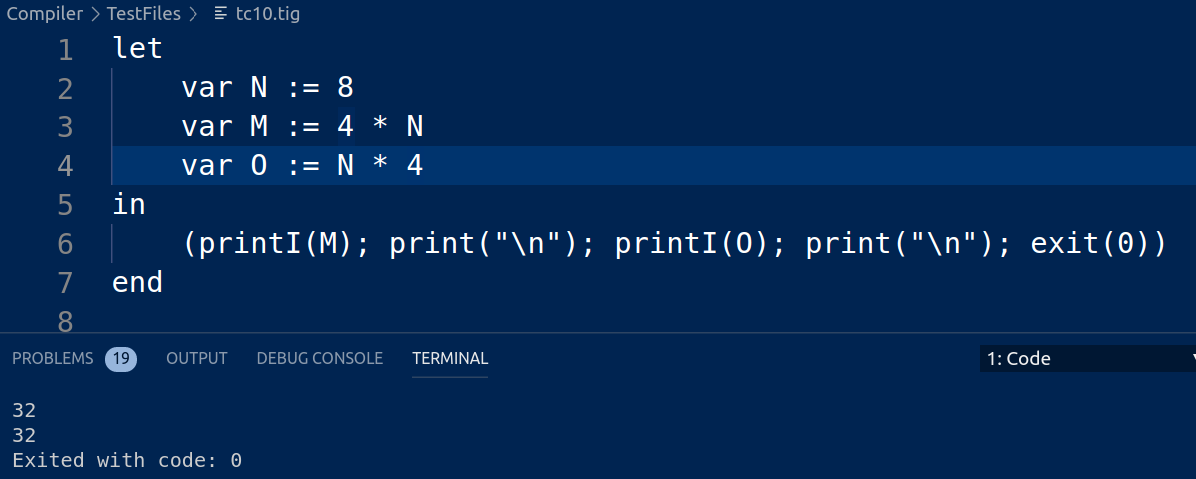
\includegraphics[width=50mm]{assets/mulopt1.png}
			      \iph{0.80}{assets/mulopt1.png}
			      \caption{Code}
			      \label{fig:mulopt1}
		      \end{subfigure}
		      \begin{subfigure}[t]{0.8\textwidth}
			      \centering
			      % 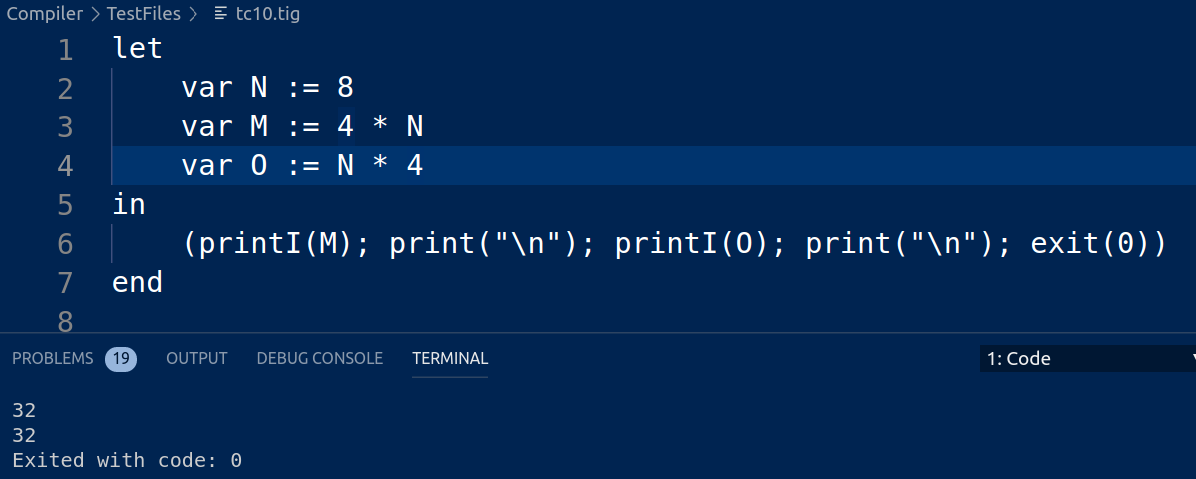
\includegraphics[width=50mm]{assets/mulopt1.png}
			      \iph{0.70}{assets/mulopt2.png}
			      \caption{\texttt{mul} statements replaced with \texttt{sll}}
			      \label{fig:mulopt2}
		      \end{subfigure}
		      \caption{Multiplication Optimization}
	      \end{figure}
	\item Started work on giving a guess of literal in case of small typo.
	      \begin{itemize}
		      \item Thinking of printing suggestions which are atmost 2 \href{https://en.wikipedia.org/wiki/Edit_distance}{distance} apart. This will bring the time complexity of standard DP approach of $O(n^2)$ to just $O(n)$.
		      \item Currently the issue is that to implement this, I would have to do lots of modification of the current code. Although I have \href{https://github.com/sourabh2311/btp/commit/8f27478a3c51b9e41bef68961a28c400d4ef29dd}{abstracted} out \textit{Not Found} error messages out with the environment, what is just left is to compare the literal with those of nearby length in the environment.
		      \item But to efficiently get those strings of nearby length there should be a map which maps lengths to the string set. (An array indexed by length may as well be used) To do this, I would have to define additional data structures and put them at appropriate place.
		      \item The main issue is that in the current design, environment just have integers mapped to environment entry. We got this integer by mapping string to counter, not storing the reverse map. This can be worked around by using \href{http://www.cs.utah.edu/~mjones/sml-nj-lib/atom.html}{Atom}.
	      \end{itemize}
	\item Started work on improving my Register Allocator. Current version is a bit simplified version of the algorithm mentioned in the text and is without coalescing.
\end{enumerate}

\section{Road Ahead}

Some among many possible improvements are mentioned below:-

\begin{itemize}
	\item Current implementation of register allocation isn't completely as what is given in the book. My register allocator lacks coalescing and is therefore incomplete. This algorithm was written in hurry last semester and is to be implemented with better heuristics.
	\item Basic blocks has to optimized with optimizations like constant propagation, constant folding, strength reduction etc.
	\item Error messages has to improved in semantic phase. Possible improvement can be to give suggestion for basic typos.
	\item String comparison has to be made as simple as "str1 $>$ str2", etc.,  instead of calling the string comparison functions to determine it.
	\item To implement ability to include pre-written code (header) files.
	\item To implement garbage collection.
	\item To implement dataflow analyses such as reaching definitions and available expressions and use them to implement some of the optimizations.
	\item To implement first-class function values in Tiger, so that functions can be passed as arguments and returned as results.
	\item Add support for compile time (initial) arguments.
	\item Implement floating point support.
	\item And much more is possible, its like in a product.
\end{itemize}

\cleardoublepage 
\typeout{}
\chapter{Introduction to RISC V and runtime.s}

\section{Choosing a Simulator}

In case of MIPS, it was straight forward to compile and run the assembly code but in case of RISC V, I had to struggle for some time as I couldn't find an appropriate documentation for it. After many iterations, I found the most suitable simulator, namely, \href{https://github.com/TheThirdOne/rars}{Rars}.

Please see the corresponding description of system calls \href{https://github.com/TheThirdOne/rars/wiki/Environment-Calls}{here}. It as well have a nice companion \href{https://github.com/TheThirdOne/rars/wiki}{documentation} which I expect one to read before proceeding further with the report.

There are other ways to compile and run RISC V code:

\begin{itemize}

  \item \href{http://www.kvakil.me/venus/}{Venus}, \href{https://github.com/kvakil/venus}{Github repo}. Note that for system calls, their argument register is different, see \href{https://github.com/TheThirdOne/rars/issues/45}{this}. 

  \item \texttt{spike} (sort of an official simulator), installed when using \texttt{riscv-gnu-toolchain}. Note it was as well required to install \href{https://github.com/riscv/riscv-pk}{pk}. System calls are different than RARS, basically it follows linux system calls. Can see these system calls \href{https://github.com/riscv/riscv-pk/blob/master/pk/syscall.c}{here1} and \href{https://github.com/riscv/riscv-pk/blob/master/pk/syscall.h}{here2}. And linux system calls \href{http://man7.org/linux/man-pages/man2/syscalls.2.html}{here}, note that system calls of interest can be concisely seen \href{https://rv8.io/syscalls.html}{here}.
  
  So to compile and run the program, do: (Don't know if this is the intended way but after a lot of trial and error, I found this)
  
  \begin{minted}{bash}
  riscv64-unknown-elf-as -o filename.o filename.s 
  riscv64-unknown-elf-ld -o filename filename.o 
  spike pk filename
  \end{minted}

\end{itemize}

\section{Basic Examples}

Few things to keep in mind:

\begin{itemize}
  \item Note that dont use \texttt{\$reg}, instead simply use \texttt{reg}.
  \item Always have two sections, one for data and another for text.
  \item During \texttt{ecall} all registers besides the output are guaranteed not to change.
  \item Put return value in \texttt{a0}.
  \item When we want our register value to be saved across system call, we can simply put it in stack instead of using registers $s_i$ as anyway we would have to save their value first in stack so no change in overhead.
  \item \texttt{a7} is used to tell which system call.
  \item Save \texttt{ra} register if executing \texttt{jal} inside a function.
\end{itemize}

\subsubsection{Hello World}

\begin{minted}{asm}
.data # Tell the assembler we are defining data not code

msg: # Label this position in memory so it can be referred to in our code
  .string "hello world" # Copy the string "hello world" into memory 

.text # Tell the assembler that we are writing code (text) now 

start:
  li a7, 4 # li means to Load Immediate and we want to load the value 4 into register a7
  la a0, msg  # la is similar to li, but works for loading addresses
  ecall
  li a7, 10  # Exit call
  ecall
\end{minted}

To get the same code working using spike. 

\begin{minted}{asm}
.globl _start # We must need to give _start, .globl helps to see it outside this file
.data 
str:   
  .string "Hello World!\n" 

.text 
_start: 

  li a0, 1   
  la a1, str 
  li a2, 13  # length of the string as required for linux system call. We can write a function which will determine the length of the string by checking for terminating null character.
  li a7, 64  
  ecall 

  li a0, 0   # The exit code we will be returning is 0
  li a7, 93  # Again we need to indicate what system call we are making and this time we are calling exit(93)
  ecall 
\end{minted}

\subsubsection{Saving callee save registers}
\begin{minted}{asm}
.data

  bef: .string "Before modification, value is: "
  dur: .string "\nInside function, value is: "
  aft: .string "\nAfter function call, value is: "

.text 

main:
  addi s0, zero, 1
  # Print bef
  la a0, bef
  li a7, 4
  ecall
  # Print int
  li a7, 1
  mv a0, s0
  ecall
  jal increment
  # Print aft
  la a0, aft
  li a7, 4
  ecall
  # Print int
  li a7, 1
  mv a0, s0
  ecall
  # Exit
  li a7, 10
  ecall



increment:
  addi sp, sp, -4
  sw s0, 0(sp) # '0' denotes the offset, in case of 0, we can simply omit it.
  addi s0, s0, 1
  # Print string
  la a0, dur
  li a7, 4
  ecall
  # Print the incremented integer
  mv a0, s0
  li a7, 1
  ecall
  lw s0, 0(sp)
  addi sp, sp, 4
  jr ra
\end{minted}

\section{runtime.s}

There are some standard functions which our Tiger program can use. They are written in \texttt{runtime.s}. I could have as well used \href{https://www.cs.princeton.edu/~appel/modern/spim/runtime.s}{file} provided by author but as I want to augment it further and implement things my way, I decided to write runtime myself. Each of the functions of runtime is explained below along with code for easy understanding. 

\begin{minted}{asm}
.data 

__exitMessage: .string "Exited with code: "
__newLine: .string "\n"

.text

# Many of the below written functions assume that the given input is correct. 

# Given the exit code (in a0 ofc), terminate with that exit code.
exit:
    mv t0, a0
    # Print exit message
    la a0, __exitMessage
    li a7, 4 
    ecall 
    # Print code
    mv a0, t0 
    li a7, 1 
    ecall 
    # Print new line
    la a0, __newLine 
    li a7, 4 
    ecall  
    # Exit
    li a7, 10
    ecall

# Not of non zero integer is 0 whereas not of 0 is 1.
not:
    beqz a0, retOne
    li a0, 0
    jr ra 
    retOne:
        li a0, 1
        jr ra 

# Given the string s in a0, return the number of characters in it.
# This is aswell needed for string concatenation.
size:
    mv t0, a0
    mv a0, zero
    sizeLoop:
        lb t1, (t0)
        beqz t1, sizeExit
        addi a0, a0, 1
        addi t0, t0, 1
        j sizeLoop
    sizeExit:
        jr ra

# Copy the string completely (i.e. including zero / null character) whose address is at a1, to the address starting at a0, returning the address of the last character of copied string.
stringCopy:
    stringCopyLoop:
        lb t0, (a1)
        sb t0, (a0)
        beqz t0, stringCopyExit
        addi a0, a0, 1
        addi a1, a1, 1
        j stringCopyLoop
    stringCopyExit:
        jr ra

# Concatenate str1 present in a0 with str2 present in a1.
concat:
    addi sp, sp, -12
    sw a0, (sp)
    sw a1, 4(sp)
    sw ra, 8(sp)
    jal size
    li t0, 1  # Will contain len(str1) + len(str2) + 1. '+1' for null character.
    add t0, t0, a0
    addi sp, sp, -4
    sw t0, (sp)
    lw a0, 8(sp)  # offset is changed
    jal size
    lw t0, (sp)
    add t0, t0, a0
    addi sp, sp, 4
    mv a0, t0
    li a7, 9
    ecall
    addi sp, sp, -4
    sw a0, (sp)
    lw a1, 4(sp)
    jal stringCopy
    lw a1, 8(sp)
    jal stringCopy
    lw a0, (sp)
    lw ra, 12(sp)
    addi sp, sp, 16
    jr ra

# "function substring (s: string, first : int, n : int) : string" Substring of string s, starting with character first, n characters long.
# Hoping that given input is valid.
substring:
    # Allocate space
    mv a3, a0  # saving a0
    mv a0, a2
    addi a0, a0, 1  # for null character 
    li a7, 9
    ecall
    # making a3 point to the desired substring
    add a3, a3, a1 
    mv t0, a0  # we need to return this
    substringLoop:
        lb t1, (a3) 
        sb t1, (a0)
        beqz a2, substringExit
        addi a0, a0, 1 
        addi a3, a3, 1
        addi a2, a2, -1
        j substringLoop
    substringExit: 
        mv a0, t0
        jr ra

# str1 > str2 ?
stringGreat:
    stringGreatLoop:
        lb a2 (a0)
        lb a3 (a1)
        bgt a2, a3  stringGreatA
        blt a2, a3  stringGreatB
        # If we have reached this point that means both are equal and if one of them is zero that means other is aswell 0, so in case strings are equal, I must return 0.
        beqz a2, stringGreatB
        addi a0, a0, 1
        addi a1, a1, 1
        j stringGreatLoop
    stringGreatA:
        li a0, 1
        jr ra
    stringGreatB:
        li a0, 0 
        jr ra 
    
# str1 < str2 ?
stringLess:
    stringLessLoop:
        lb a2 (a0)
        lb a3 (a1)
        blt a2, a3  stringLessA
        bgt a2, a3  stringLessB
        # If we have reached this point that means both are equal and if one of them is zero that means other is aswell 0, so in case strings are equal, I must return 0.
        beqz a2, stringLessB
        addi a0, a0, 1
        addi a1, a1, 1
        j stringLessLoop
    stringLessA:
        li a0, 1
        jr ra
    stringLessB:
        li a0, 0 
        jr ra 

# str1 == str2 ?
stringEqual:
    addi sp, sp, -12
    sw a0, (sp)
    sw a1, 4(sp)
    sw ra, 8(sp)
    jal stringGreat
    bnez a0, stringEqualExit
    lw a0, (sp)
    lw a1, 4(sp)
    jal stringLess
    bnez a0, stringEqualExit 
    li a0, 1 
    lw ra, 8(sp)
    addi sp, sp, 12 
    jr ra 
    stringEqualExit:
        li a0, 0    
        lw ra, 8(sp)
        addi sp, sp, 12 
        jr ra 


# Single-character string from ASCII value given in a0; halt program if a0 out of range.
chr:
    # Handling the error part 
    addi t0, zero, 127  
    bgt a0, t0, chrError
    bltz a0, chrError
    # Allocating
    mv t0, a0 
    li a0, 2 
    li a7, 9 
    ecall 
    # Putting the character
    sb t0 (a0)
    sb zero 1(a0)
    jr ra
    chrError:
        addi a0, zero, -1
        j exit

# Given a string in a0, return ASCII value of the first character of it, return -1 if the string is empty.
ord:
    lb t0, (a0)
    beqz t0, ordEmpty
    mv a0, t0 
    jr ra 
    ordEmpty:
        li a0, -1 
        jr ra 

# Read a character from standard input and return it as a string; return empty string on end of file.
getchar:
    # Allocate space
    li a0, 2
    li a7, 9
    ecall
    sb zero, 1(a0)  # Null character 
    # Read the character 
    mv t0, a0 
    li a7, 12 
    ecall 
    sb a0, (t0)  # Store the character 
    mv a0, t0 
    jr ra

# Absolete as of now
flush:
    jr ra

# Print the string whose address is in a0
print:
    li a7, 4
    ecall
    jr ra

# printInt:
#     # Examples in book do complex computation to print an integer, here I am putting an inbuilt function
#     # Print the integer in a0
#     li a7, 1
#     ecall
#     jr ra

# a0 contains the number of bytes we need to allocate. So, multiply it by 4 and allocate that much space from heap (system call 9). Return value is in a0 which tells the address to the allocated block (lower address value) and remember that in going downwards address decreases. Rest of the code is easy to follow. Note that a1 contains the value to which we need to initialize our array.
initArray:
  li t0, 4
  mul a0, a0, t0
    mv t1, a0
  li a7, 9
  ecall
  mv t0, a0
  add t1, t1, t0
  initArrayLoop:
        sw a1, (t0)
        addi t0, t0, 4
        beq t0, t1, initArrayExit
        j initArrayLoop
    initArrayExit:
        jr ra

# Very similar to initArray
# We just need to allocate memory, no need to initialize it with 0.
allocRecord:
    li t0, 4
    mul a0, a0, t0
    li a7, 9
    ecall
    jr ra
\end{minted}
\cleardoublepage 
\typeout{}
\chapter{Phase I : Constructing Abstract Syntax Tree}

In this phase, files of interest are:-

\begin{itemize}
  \item \href{\git parse.sml}{parse.sml}
  \item \href{\git errormsg.sml}{errormsg.sml}
  \item \href{\git tiger.lex}{tiger.lex}
  \item \href{\git table.sml}{table.sml}, \href{\git table.sig}{table.sig}
  \item \href{\git symbol.sml}{symbol.sml} 
  \item \href{\git tiger.grm}{tiger.grm}, \href{\git absyn.sml}{absyn.sml} 
\end{itemize}

Each of these is explained below.

\section{parse.sml}

We know the compiler follows "Lexical Analysis $\rightarrow$ Parsing $\rightarrow$ \dots". \texttt{parse.sml} is the one which does these two and ties the various files associated with it and finally returns the desired abstract syntax tree.

\section{errormsg.sml}

Besides errors encountered in lexical analysis phase, they'll be print using \texttt{errormsg.sml} which will print these errors in an elaborate manner.

I'll be explaining the signature of this file here, which is sufficient to understand the working of this file.

\begin{minted}{sml}
(* In our lexer, each line will occur at a particular "pos" which is incremented for each character ("pos" is nothing but the number of characters read till now). For each line, we maintain its "pos". Our goal is that given "pos", we have to determine the line number and column number, this can now be easily done, just determine that line with maximum "pos" which is less than the given "pos", the difference now gives the column number. Reason of doing this in such an odd way is because in our grammar, lexer and in abstract syntax file we define "pos" to be int and not as a tuple (int, int) where first parameter could denote line number and other one as column number. *)

signature ERRORMSG =
sig
    val anyErrors : bool ref  (* has their been an occurance of any error? *)
    val fileName : string ref (* Updated in parse.sml, used when printing errors *)
    val lineNum : int ref (* Number of lines in the read file *)
    val linePos : int list ref (* as defined in the top most comment, it is the list containing value of "pos" at each line *)
    val error : int -> string -> unit (* it should take "pos" and error message to print, from "pos" it will determine the line number and the column number, and will print abstractly "filename:lineNo.ColNo:Message". *)
    exception Error
    val impossible : string -> 'a   (* raises Error, for a behavior we didn't expect *)
    val reset : unit -> unit  (* reset the parameters, so that we can move on to read new file *)
end
\end{minted}

\section{tiger.lex}

Simple lexer for our language, just that for some of the errors like non terminated string, etc. are easily detected in this phase and thus are printed now with putting an end to the compilation phase. Usually one detects many errors and print them all instead of just printing one error and stopping. But I feel that errors in lexical phase, if found, are critical and should be handled first most. 

\subsubsection{Guidelines}

Few important rules to keep in mind:

\begin{itemize}
  \item Longest match: The longest initial substring of the input that can match any regular expression is taken as the next token.
  \item Rule priority: For a particular longest initial substring, the first regular expression that can match determines its token type. This means that the order of writing down the regular-expression rules has significance.
  \item An individual character stands for itself, except for the reserved characters 
    \begin{minted}{cpp}
     ? * + | ( ) ^ / ; . = < > [ { " \  $
    \end{minted}
  \item A backslash followed by one of the reserved characters stands for that character. 
  \item Inside the brackets, only the symbols 
  \begin{minted}{cpp} 
    \ - ^ 
  \end{minted}
    are reserved. An initial up-arrow \^{} stands for the complement of the characters listed, e.g. [\^{}abc] stands any character except a, b, or c.
  \item  To include \^{} literally in a bracketed set, put it anywhere but first; to include - literally in a set, put it first or last. 
  \item The dot . character stands for any character except newline, i.e. the same as 
  \begin{minted}{cpp}
    [^\n]
  \end{minted}
  \item The following special escape sequences are available, inside or outside of square brackets: 
    \begin{minted}{SML}
    \b backspace
    \n newline
    \t horizontal tab
    \ddd where ddd is a 3 digit decimal escape
    \end{minted}
    \item Any regular expression may be enclosed in parentheses ( ) for syntactic (but, as
    usual, not semantic) effect
    \item A sequence of characters will stand for itself (reserved characters will be taken literally) if it is enclosed in double quotes " ".
    \item A postfix repetition range \{a, b\} where a and b are small integers stands for any number of repetitions between a and b of the preceding expression. The notation \{a\} stands for exactly a repetitions. Ex: [0-9]\{3\}
    Any three-digit decimal number. 
    \item The rules should match all possible input. If some input occurs that does not match any rule, the lexer created by ML-Lex will raise an exception LexError.
\end{itemize}

\section{table.sml, table.sig}

For our immediate steps, we would need a way to map our "keys" to a particular "value", for this we create a functor, "IntMapTable" which takes the type of "key" and a function to get an integer corresponding to that "key". Then this functor uses "IntBinaryMap", a hash map to represent our map. This "IntBinaryMap" is polymorphic, so we can use it for any value corresponding to our int (which we obtained from our key). This is the purpose served by "table.sig" and "table.sml". 

\section{symbol.sml}

Each of the variable, function declaration etc. will be stored as "symbols" (a pair of (string, int)). Where each symbol will have a unique integer. We can then map this integer to anything using our "IntBinaryMap". Purpose of keeping this symbols is that we would like to see whether this variable is declared before or not, whether this type exists or not, etc.

\section{tiger.grm, absyn.sml}

\texttt{tiger.grm} is the parser for our language, it will read the tokens from lexer and build AST using \texttt{absyn.sml}. Grammar directly follows the rules given in the book. 

\subsubsection{Guidelines}

\begin{itemize}
  \item Format of ML-YACC: user declarations \%\% parser declarations \%\% grammar rules.
  \item By default, ML-YACC resolves shift-reduce conflicts by shifting, and reduce-reduce conflicts by using the rule that appears earlier in the grammar. If then (else) shift-reduce conflict is thus not harmful.
  \item Consider for example: 
  \begin{minted}{bash}
  E -> E * E.   (+)
  E -> E. + E   (any)
  \end{minted}
  The precedence declarations (\%left, etc.) give priorities to the tokens; the priority of a rule is given by the last token occurring on the right-hand side of that rule. Thus the choice here is between a rule with priority "*" and a token with priority "+"; the rule has higher priority, so the conflict is resolved in favor of reducing.
  \item When the rule and token have equal priority, then a \%left precedence favors reducing, \%right favors shifting, and \%nonassoc yields an error action.
  \item Instead of using the default "rule has precedence of its last token," we can assign a specific precedence to a rule using the \%prec directive. This is commonly used to solve the "unary minus" problem. In most programming languages a unary minus binds tighter than any binary operator, so —6 * 8 is parsed as (—6) * 8, not —(6 * 8).
  \item Precedence declaration should be written in the order of increasing precedence. 
\end{itemize}

For more description, please see the comments in the file \texttt{tiger.grm}.
\cleardoublepage 
\typeout{}
\chapter{Phase II : Constructing Intermediate Representation Tree}

Now that we have constructed our Abstract Syntax Tree, we will now have to convert it to an Intermediate Representation to solve $m \times n$ problem and also code generation would be easy on this language as it is more close to many machine languages.

\section{Type Interface}

\tfbox{\href{\git types.sml}{types.sml}}

Our next step is to do type checking of our input AST. For this purpose we need to define auxiliary types. Thus, we have \texttt{types.sml} representing the same. Thus now we can easily map a "symbol" to its corresponding type.

\section{Types/Variables Environment}

\tfbox{\href{\git env.sml}{env.sml} \\ \href{\git env.sig}{env.sig} \\ \href{\git temp.sml}{temp.sml} \\ \href{\git temp.sig}{temp.sig}}

Now for type checking, we need some environment under which we have to check compatibility of types as for instance, environment can be different for different functions as within \texttt{let} block of each function there can be new declarations etc. By default we have some standard types and functions already present in our environment and are thus listed in \texttt{env.sml}. Now each of these functions will correspond to some label in our MIPS code, for which we have \texttt{temp.sml}. Note that \texttt{temp.sml} is also used to represent our infinite register in Intermediate Representation.

\section{Finding Escaped Variables}

\tfbox{\href{\git findescape.sml}{findescape.sml}}

It would be important for us to determine which variable cannot go to a register, i.e., which variable escapes. Idea of finding escapes is straight forward: Just see if this thing was defined in outer scope, note that scope extends only when we are calling a function. Escaping is calculated in \texttt{findescape.sml}

\section{Intermediate Tree Representation}

\tfbox{\href{\git tree.sml}{tree.sml} \\ \href{\git tree.sig}{tree.sig}}

The files \texttt{tree.sml, tree.sig} consists of datatype representing our Intermediate Tree. Description of which is presented as below.

\begin{minted}{sml}
  datatype stm = SEQ of stm * stm (* The statement s2 followed by s2. *)
  | LABEL of label (* Define the constant value of name n to be the current machine code address. This is like a label definition in assembly language. *)
  | JUMP of exp * label list (* Transfer control (jump) to address exp. The destination exp may be a literal label, as in NAME(lab), or it may be an address calculated by any other kind of expression. For example, a C-language switch (i) statement may be implemented by doing arithmetic on i. The list of labels labs specifies all the possible locations that the expression exp can evaluate to; this is necessary for dataflow analysis later. The common case of jumping to a known label "l" is written as jump(name l, [l]). *)
  | CJUMP of relop * exp * exp * label * label (* CJUMP(o, e1, e2, t, f): Evaluate e1, e2 in that order, yielding values a, b. Then compare a, b using the relational operator o. If the result is true, jump to t otherwise jump to f. The relational operators *)
  | MOVE of exp * exp 
  (*
     MOVE(TEMP t, e): Evaluate e and move it into temporary t. 
     MOVE(MEM(e1), e2) Evaluate e1 yielding address a. Then evaluate e2 and store the result into wordSize bytes of memory starting at a.
  *)
  | RMOVE of exp * exp (* same as above but for reals *)
  | EXP of exp (* Evaluate exp and discard the result. *)

and exp = BINOP of binop * exp * exp (* The application of binary operators to operands exp1, exp2. *)
  | MEM of exp (* The contents of wordSize bytes of memory starting at address exp (where wordSize is defined in the Frame module). Note that when MEM is used as the left child of a move, it means "store," but anywhere else it means "fetch." *)
  | RMEM of exp (* same as above but for reals *)
  | TEMP of Temp.temp (* Temporary t. A temporary in the abstract machine is similar to a register in a real machine. However, the abstract machine has an infinite number of temporaries. *)
  | ESEQ of stm * exp (* The statement s is evaluated for side effects, then e is evaluated for result *)
  | NAME of label (* The value NAME(n) may be the target of jumps, calls, etc. *)
  | CONST of int (* The integer constant int. *)
  | CALL of exp * exp list (* A procedure call: the application of function exp1 to argument list exp2 list. The subexpression exp1 is evaluated before the arguments which are evaluated left to right. *)

and binop = PLUS | MINUS | MUL | DIV | AND | OR | LSHIFT | RSHIFT | ARSHIFT | XOR

and relop = EQ | NE | LT | GT | LE | GE | ULT | ULE | UGT | UGE
\end{minted}

\section{Understanding Functions Calls in Tiger}

\nbox{Some of this material will become clear after reading Phase III.}

\begin{figure}
	\centering
	\iph{0.35}{assets/myFrame.png}
	\caption{Illustration of Frame}
	\label{fig:myframe}
\end{figure}

Below is explained in chronological sequence of what happens and for
what reason when function call is executed in this compiler. Also see \ref{fig:myframe}.

\begin{enumerate}
	\def\labelenumi{\arabic{enumi}.}
	\item
	      When a function is called. The current frame is extended to include
	      outgoing parameters (at the offset already determined by the callee)
	      in case some of them escape; rest of the arguments are put in argument
	      registers.

	      \begin{enumerate}
		      \def\labelenumii{\arabic{enumii}.}
		      \item
		            This step is done by our code generator.
		      \item
		            After moving escaped arguments to their pre-determined location and
		            remaining arguments to argument registers, it will then emit
		            \mintinline[breaklines=true, tabsize=2, breaksymbolleft=]{text}{jal}
		            instruction which will have
		            \mintinline[breaklines=true, tabsize=2, breaksymbolleft=]{text}{src = argTemps}
		            (\mintinline[breaklines=true, tabsize=2, breaksymbolleft=]{text}{argTemps}
		            are chosen argument registers, this is done as these argument
		            registers are used in this time) and
		            \mintinline[breaklines=true, tabsize=2, breaksymbolleft=]{text}{dst = [ra] @ F.getFirstL F.callersaves};
		            as we know that caller is supposed to save some registers if it was
		            using them and thus setting
		            \mintinline[breaklines=true, tabsize=2, breaksymbolleft=]{text}{dst = F.getFirstL F.callersaves}
		            would enable the garbage collection to know that if function being
		            called \textbf{uses} these registers then it would clearly
		            interfere. For all but those functions which are at top most, we as well pass the static link for the function enclosing the called function. Please see the example code in the text.
		      \item
		            Let
		            \mintinline[breaklines=true, tabsize=2, breaksymbolleft=]{text}{fp},
		            \mintinline[breaklines=true, tabsize=2, breaksymbolleft=]{text}{sp}
		            denote the current frame and stack pointer.
		      \item
		            To extend the current frame, we must subtract it by the amount
		            \mintinline[breaklines=true, tabsize=2, breaksymbolleft=]{text}{escaped-arguments * word-size}.
		            But since we should as well store the old frame pointer (as we will
		            update it with the current stack pointer, this frame pointer is not same as static link); we must subtract
		            \mintinline[breaklines=true, tabsize=2, breaksymbolleft=]{text}{sp}
		            by
		            \mintinline[breaklines=true, tabsize=2, breaksymbolleft=]{text}{(escaped-arguments + 1) * word-size}.
		      \item
		            Now old value of fp is saved in 0th location of this
		            \mintinline[breaklines=true, tabsize=2, breaksymbolleft=]{text}{sp},
		            and other arguments are saved respectively at the offsets already
		            determined by the callee. (Callee predetermined these offsets
		            considering the fact that we will save old
		            \mintinline[breaklines=true, tabsize=2, breaksymbolleft=]{text}{fp}
		            at 0th word)
		      \item
		            Now as we are moving to the frame of other function
		            \mintinline[breaklines=true, tabsize=2, breaksymbolleft=]{text}{fp}
		            is updated to
		            \mintinline[breaklines=true, tabsize=2, breaksymbolleft=]{text}{sp},
		            and
		            \mintinline[breaklines=true, tabsize=2, breaksymbolleft=]{text}{sp}
		            value will be deducted by the amount needed by the callee stack.
		      \item
		            Thus local variables allocated will be referred with negative offset
		            wrt to
		            \mintinline[breaklines=true, tabsize=2, breaksymbolleft=]{text}{fp}
		            and escaped argument parameters will be referred with non negative
		            offset wrt
		            \mintinline[breaklines=true, tabsize=2, breaksymbolleft=]{text}{fp}.
		      \item
		            Thus it is evident that our code generator would need to know the
		            access list of the callee which wasn't there in the design mentioned
		            in the book, so I added it in
		            \mintinline[breaklines=true, tabsize=2, breaksymbolleft=]{text}{tree.sml}
		            but to avoid cyclic dependency between
		            \mintinline[breaklines=true, tabsize=2, breaksymbolleft=]{text}{tree.sml}
		            and
		            \mintinline[breaklines=true, tabsize=2, breaksymbolleft=]{text}{riscframe.sml},
		            I had to redefine
		            \mintinline[breaklines=true, tabsize=2, breaksymbolleft=]{text}{access}
		            and had to create
		            \mintinline[breaklines=true, tabsize=2, breaksymbolleft=]{text}{accessConv.sml}
		            to facilitate conversion between access of
		            \mintinline[breaklines=true, tabsize=2, breaksymbolleft=]{text}{tree}
		            and
		            \mintinline[breaklines=true, tabsize=2, breaksymbolleft=]{text}{riscframe}.
		      \item
		            Also since code generator must save escaped arguments with respect
		            to the new frame pointer which is not equal to current frame pointer
		            as this whole thing is updated in
		            \mintinline[breaklines=true, tabsize=2, breaksymbolleft=]{text}{procEntryExit3},
		            but since new frame pointer = current stack pointer - (escape-count
		            + 1) * word-size, I created new function
		            \mintinline[breaklines=true, tabsize=2, breaksymbolleft=]{text}{callexp}
		            in
		            \mintinline[breaklines=true, tabsize=2, breaksymbolleft=]{text}{riscframe}
		            to do this arithmetic.
	      \end{enumerate}
	\item
	      Now inside this called function, we must create new temporary for each
	      passed argument \textbf{in argument register} and move that register's
	      value to this new temporary. This might seem unnecessary but consider
	      \mintinline[breaklines=true, tabsize=2, breaksymbolleft=]{text}{function m(x : int, y : int) = (h(y, y); h(x, x))}.
	      If \mintinline[breaklines=true, tabsize=2, breaksymbolleft=]{text}{x}
	      stays in ``parameter register 1'' throughout
	      \mintinline[breaklines=true, tabsize=2, breaksymbolleft=]{text}{m},
	      and \mintinline[breaklines=true, tabsize=2, breaksymbolleft=]{text}{y}
	      is passed to
	      \mintinline[breaklines=true, tabsize=2, breaksymbolleft=]{text}{h} in
	      parameter register 1, then there is a problem. The register allocator
	      will eventually choose which machine register should hold the
	      temporary. If there is no interference of the type shown in function
	      \mintinline[breaklines=true, tabsize=2, breaksymbolleft=]{text}{m},
	      then (on the RISC) the allocator will take care to choose register the
	      same register as temporary to hold that register (not implemented as of now). Then the move
	      instructions will be unnecessary and will be deleted at that time.

	      \begin{itemize}
		      \item
		            This is done in
		            \mintinline[breaklines=true, tabsize=2, breaksymbolleft=]{text}{newFrame}
		            of
		            \mintinline[breaklines=true, tabsize=2, breaksymbolleft=]{text}{riscframe},
		            named as
		            \mintinline[breaklines=true, tabsize=2, breaksymbolleft=]{text}{shiftInstr}
		            (shift instructions).
	      \end{itemize}
	\item
	      Called function must save callee-save registers include
	      \mintinline[breaklines=true, tabsize=2, breaksymbolleft=]{text}{ra},
	      this is done in
	      \mintinline[breaklines=true, tabsize=2, breaksymbolleft=]{text}{procEntryExit1},
	      similarly restoring them in the end of function body is as well done
	      here.
\end{enumerate}

\section{RISC Frame}

\tfbox{\href{\git riscframe.sml}{riscframe.sml}}

File \texttt{riscframe.sml} contains an interface for RISC V, which finds some use in this phase, but is mainly there for code generation phase. Its applications and purpose will become clear by seeing the written code. Before proceeding please read and understand about \textbf{static links} given at page 132-134 of the \textit{Tiger Book}\cite{tigerbook}. Basic gist is that in languages that allow nested function declarations, the inner functions may use variables declared in outer functions. One way to accomplish this is that whenever a function $f$ is called, it can be passed a pointer to the frame of the function statically enclosing $f$; this pointer is the static link.

\section{Translating to IR}

\tfbox{\ghref{translate.sml}}

Done by \texttt{translate.sml} and is used by \texttt{semant.sml} to generate IR tree code.

\texttt{semant.sml} will generate an \texttt{exp} of translate type for a frame and then in the end, it will call translate's \texttt{procEntryExit} which will \texttt{unEx} that expression.


Its not reasonable to translate expression of our AST to an expression of IR as this is true only for certain kinds of expressions, the ones that  compute a value. Expressions that return no value (such as some procedure calls, or while expressions in the Tiger language) are more naturally represented by \texttt{Tree.stm}. And expressions with Boolean values, such as $a > b$, might best be represented as a conditional jump - a combination of \texttt{Tree.stm} and a pair of destinations represented by \texttt{Temp.labels}. Therefore, we will make a datatype exp in the Translate module to model these three kinds of expressions:

\begin{minted}{sml}
datatype exp =  Ex of Tr.exp
							| Nx of Tr.stm
              | Cx of Temp.label * Temp.label -> Tr.stm
\end{minted}

\begin{itemize}

	\item \textbf{Ex} stands for an "expression," represented as a \texttt{Tree.exp}.
	\item \textbf{Nx} stands for "no result," represented as a Tree statement.
	\item \textbf{Cx} stands for "conditional," represented as a function from label-pair to  statement. If you pass it a true-destination and a false-destination, it will make a statement that evaluates some conditionals and then jumps to one of the  destinations (the statement will never "fall through"). For example, the Tiger expression
	      \begin{minted}{sml}
  a > b | c < d
  \end{minted}
	      might translate to the  conditional:
	      \begin{minted}{sml}
  Cx(fn (t,f) => SEQ(CJUMP(GT, a, b, t, z),
  SEQ(LABEL z, CJUMP (LT, c, d, t, f))))
  \end{minted}
	      for some new label \texttt{z}.
\end{itemize}

Sometimes we will have an expression of one kind and we will need to convert it to an equivalent expression of another kind. For example, the Tiger statement
\begin{minted}{sml}
flag := (a>b | c<d)
\end{minted}
. This is achieved by \texttt{unEx}. Similarly we have \texttt{unNx} and \texttt{unCx}.

Similarly each function call defines a level which is encapsulated as
\begin{minted}{sml}
datatype level =  Top
                | Lev of {parent: level, frame: F.frame} * unit ref
\end{minted}

\texttt{unit ref} is used to easily check for equality.

All of the functions of \texttt{translate.sml} are straight forward so please see and understand them.

\section{Semantic Analysis}

\tfbox{\ghref{semant.sml}}

After we receive our AST, we run semant's (in \texttt{semant.sml}) function \texttt{transProg} on it which will do type checking of our AST and simultaneously convert it into our IR. Both this and \texttt{translate.sml} are big so I have not put their code here, however please see linked code which is properly documented and thus is easy to understand.
\cleardoublepage 
\typeout{}
\chapter{Phase III : Generating Assembly Code}

This final phase generates the machine assembly code and thus completing the purpose of compiler. 
It involves the discussion of various concepts such as Canonisation, Instruction Selection, Liveness Analysis and Register Allocation.

Each of these is explained in an understandable order below.

\section{Canonisation}

\tfbox{\ghref{canon.sml}}

\hypertarget{abstract}{%
\subsection{Abstract}\label{abstract}}

It's useful to be able to evaluate the sub-expressions of an expression
in any order. If tree expressions did not contain
\mintinline[breaklines=true, tabsize=2, breaksymbolleft=]{text}{ESEQ}
and
\mintinline[breaklines=true, tabsize=2, breaksymbolleft=]{text}{CALL}
nodes, then the order of evaluation would not matter.

\hypertarget{why-call-nodes-are-an-issue}{%
\subsubsection{\texorpdfstring{Why
\mintinline[breaklines=true, tabsize=2, breaksymbolleft=]{text}{CALL}
nodes are an
issue?}{Why  nodes are an issue?}}\label{why-call-nodes-are-an-issue}}

In actual implementation,
\mintinline[breaklines=true, tabsize=2, breaksymbolleft=]{text}{CALL}
nodes will return value in the same register
(\mintinline[breaklines=true, tabsize=2, breaksymbolleft=]{text}{a0} in
case of RISC V). Thus in an expression like
\mintinline[breaklines=true, tabsize=2, breaksymbolleft=]{text}{BINOP(PLUS, CALL(...), CALL(...))};
the second call will overwrite the
\mintinline[breaklines=true, tabsize=2, breaksymbolleft=]{text}{a0}
register before the
\mintinline[breaklines=true, tabsize=2, breaksymbolleft=]{text}{PLUS}
can be executed.

Remedy is to do the transformation;
\mintinline[breaklines=true, tabsize=2, breaksymbolleft=]{text}{CALL(fun, args) -> ESEQ(MOVE(TEMP t, CALL(fun, args)), TEMP t)}

\hypertarget{why-eseq-nodes-are-an-issue}{%
\subsubsection{\texorpdfstring{Why
\mintinline[breaklines=true, tabsize=2, breaksymbolleft=]{text}{ESEQ}
nodes are an
issue?}{Why  nodes are an issue?}}\label{why-eseq-nodes-are-an-issue}}

Clearly in case of simple
\mintinline[breaklines=true, tabsize=2, breaksymbolleft=]{text}{ESEQ(s, e)},
statement
\mintinline[breaklines=true, tabsize=2, breaksymbolleft=]{text}{s} can
have direct or side effects on an expression
\mintinline[breaklines=true, tabsize=2, breaksymbolleft=]{text}{e}.

Remedy is as shown in figure 5.1 (basically lifting them higher and
higher until they become
\mintinline[breaklines=true, tabsize=2, breaksymbolleft=]{text}{SEQ}
nodes).

\begin{figure}
\centering
\iph{0.70}{assets/canon1.png}
\caption{ESEQ Removal}
\end{figure}

The transformation is done in three stages: First, a tree is rewritten
into a list of canonical trees without
\mintinline[breaklines=true, tabsize=2, breaksymbolleft=]{text}{SEQ} or
\mintinline[breaklines=true, tabsize=2, breaksymbolleft=]{text}{ESEQ}
nodes; then this list is grouped into a set of basic blocks, which
contain no internal jumps or labels; then the basic blocks are ordered
into a set of traces in which every
\mintinline[breaklines=true, tabsize=2, breaksymbolleft=]{text}{CJUMP}
is immediately followed by its false label. This will become clear when
seeing the well documented code.

\section{Instruction Selection}

\tfbox{\ghref{assem.sml} \\ \ghref{codegen.sml} \\ \ghref{accessConv.sml}}

\hypertarget{instruction-representation}{%
\subsection{Instruction
Representation}\label{instruction-representation}}

Now that we have done Canonisation, our compiler will now call code
generator. It will basically convert the body into assembly language
code with the restriction that we will still be using temporaries
instead of actual machine registers. In this form, source registers will
be labelled
\mintinline[breaklines=true, tabsize=2, breaksymbolleft=]{text}{`si} and
destination registers as
\mintinline[breaklines=true, tabsize=2, breaksymbolleft=]{text}{`di}. So
our each instruction would be represented as an operation string having
these
\mintinline[breaklines=true, tabsize=2, breaksymbolleft=]{text}{`si},
\mintinline[breaklines=true, tabsize=2, breaksymbolleft=]{text}{`di}'s
where
\mintinline[breaklines=true, tabsize=2, breaksymbolleft=]{text}{`si} is
indexed from
\mintinline[breaklines=true, tabsize=2, breaksymbolleft=]{text}{src}
list, and
\mintinline[breaklines=true, tabsize=2, breaksymbolleft=]{text}{`di} are
indexed from
\mintinline[breaklines=true, tabsize=2, breaksymbolleft=]{text}{dst}
list. This is captured as
\mintinline[breaklines=true, tabsize=2, breaksymbolleft=]{text}{datatype instr}
in
\href{https://www.github.com/sourabh2311/btp/tree/master/Compiler/assem.sml}{\mintinline[breaklines=true, tabsize=2, breaksymbolleft=]{text}{assem.sml}}.

\begin{minted}[breaklines=true, tabsize=2, breaksymbolleft=]{sml}
datatype instr = 
            OPER of {assem: string, dst: temp list, src: temp list, jump: label list option}
    | LABEL of {assem: string, lab: Temp.label}
    | MOVE of {assem: string,  dst: temp, src: temp}
\end{minted}

An \mintinline[breaklines=true, tabsize=2, breaksymbolleft=]{text}{OPER}
holds an assembly-language instruction
\mintinline[breaklines=true, tabsize=2, breaksymbolleft=]{text}{assem},
a list of operand registers
\mintinline[breaklines=true, tabsize=2, breaksymbolleft=]{text}{src},
and a list of result registers
\mintinline[breaklines=true, tabsize=2, breaksymbolleft=]{text}{dst}.
Either of these lists may be empty. Operations that always fall through
to the next instruction have
\mintinline[breaklines=true, tabsize=2, breaksymbolleft=]{text}{jump = NONE};
other operations have a list of ``target'' labels to which they may jump
(this list must explicitly include the next instruction if it is
possible to fall through to it).

A \mintinline[breaklines=true, tabsize=2, breaksymbolleft=]{text}{LABEL}
is a point in a program to which jumps may go. It has an
\mintinline[breaklines=true, tabsize=2, breaksymbolleft=]{text}{assem}
component showing how the label will look in the assembly-language
program, and a
\mintinline[breaklines=true, tabsize=2, breaksymbolleft=]{text}{lab}
component identifying which label-symbol was used.

A \mintinline[breaklines=true, tabsize=2, breaksymbolleft=]{text}{MOVE}
is like an
\mintinline[breaklines=true, tabsize=2, breaksymbolleft=]{text}{OPER},
but must perform only data transfer. Then, if the
\mintinline[breaklines=true, tabsize=2, breaksymbolleft=]{text}{dst} and
\mintinline[breaklines=true, tabsize=2, breaksymbolleft=]{text}{src}
temporaries are assigned to the same register, the
\mintinline[breaklines=true, tabsize=2, breaksymbolleft=]{text}{MOVE}
can later be deleted (as done in my register allocator).

\hypertarget{code-generation}{%
\subsection{Code Generation}\label{code-generation}}

Finding the appropriate machine instructions to implement a given
intermediate representation tree is the job of the instruction selection
phase of a compiler.

We can express a machine instruction as a fragment of an IR tree, called
a tree pattern as denoted in the figure below. Then instruction
selection becomes the task of tiling the tree with a minimal set of tree
patterns.

\begin{figure}
\centering
\iph{0.7}{assets/is1.png}
\caption{Tree Patterns showing arithmetic and memory instructions}
\end{figure}

The very first entry is not really an instruction, but expresses the
idea that a
\mintinline[breaklines=true, tabsize=2, breaksymbolleft=]{text}{TEMP}
node is implemented as a register, so it can ``produce a result in a
register'' without executing any instructions at all.

For each instruction, the tree-patterns it implements are shown. Some
instructions correspond to more than one tree pattern; the alternate
patterns are obtained for commutative operators (+ and *), and in some
cases where a register or constant can be zero
(\mintinline[breaklines=true, tabsize=2, breaksymbolleft=]{text}{LOAD}
and
\mintinline[breaklines=true, tabsize=2, breaksymbolleft=]{text}{STORE}).
Here we abbreviate the tree diagrams slightly:
\mintinline[breaklines=true, tabsize=2, breaksymbolleft=]{text}{BINOP(PLUS, x, y)}
nodes will be written as
\mintinline[breaklines=true, tabsize=2, breaksymbolleft=]{text}{+(x, y)},
and the actual values of
\mintinline[breaklines=true, tabsize=2, breaksymbolleft=]{text}{CONST}
and
\mintinline[breaklines=true, tabsize=2, breaksymbolleft=]{text}{TEMP}
nodes will not always be shown.

Consider the instruction
\mintinline[breaklines=true, tabsize=2, breaksymbolleft=]{text}{a[i] := x}.
Two possible tilings for this instruction is shown in the diagram.
(Remember that
\mintinline[breaklines=true, tabsize=2, breaksymbolleft=]{text}{a} is
really the frame offset of the pointer to an array)

\begin{figure}
\centering
\iph{0.7}{assets/is2.png}
\caption{A tree tiled in two ways}
\end{figure}

\hypertarget{maximal-munch-algorithm}{%
\subsection{Maximal Munch Algorithm}\label{maximal-munch-algorithm}}

Suppose we could give each kind of instruction a cost. Then we could
define an optimum tiling as the one whose tiles sum to the lowest
possible value. An optimal tiling is one where no two adjacent tiles can
be combined into a single tile of lower cost. If there is some tree
pattern that can be split into several tiles of lower combined cost,
then we should remove that pattern from our catalog of tiles before we
begin. Every optimum tiling is also optimal, but not vice versa.

The algorithm for optimal tiling is called \textbf{Maximal Munch}. It is
quite simple. Starting at the root of the tree, find the largest tile
that fits. Cover the root node - and perhaps several other nodes near
the root - with this tile, leaving several subtrees. Now repeat the same
algorithm for each subtree. As each tile is placed, the corresponding
instruction is generated. The Maximal Munch algorithm generates the
instructions in reverse order - after all, the instruction at the root
is the first to be generated, but it can only execute after the other
instructions have produced operand values in registers. The ``largest
tile'' is the one with the most nodes. If two tiles of equal size match
at the root, then the choice between them is arbitrary. Maximal Munch is
quite straightforward to implement in ML. Simply write two recursive
functions,
\mintinline[breaklines=true, tabsize=2, breaksymbolleft=]{text}{munchStm}
for statements and
\mintinline[breaklines=true, tabsize=2, breaksymbolleft=]{text}{munchExp}
for expressions. Each clause of
\mintinline[breaklines=true, tabsize=2, breaksymbolleft=]{text}{munchExp}
will match one tile. The clauses are ordered in order of tile preference
(biggest tiles first); ML's pattern-matching always chooses the first
rule that matches.

This algorithm is implemented in the file
\href{https://www.github.com/sourabh2311/btp/tree/master/Compiler/codegen.sml}{\mintinline[breaklines=true, tabsize=2, breaksymbolleft=]{text}{codegen.sml}}

\section{Liveness Analysis and Interference Graph}

\tfbox{\ghref{flowgraph.sml} \\ \ghref{makegraph.sml} \\ \ghref{liveness.sml}}

\hypertarget{liveness-analysis}{%
\subsection{Liveness Analysis}\label{liveness-analysis}}

Two temporaries
\mintinline[breaklines=true, tabsize=2, breaksymbolleft=]{text}{a} and
\mintinline[breaklines=true, tabsize=2, breaksymbolleft=]{text}{b} can
fit into the same register, if
\mintinline[breaklines=true, tabsize=2, breaksymbolleft=]{text}{a} and
\mintinline[breaklines=true, tabsize=2, breaksymbolleft=]{text}{b} are
never ``in use'' at the same time.

We say a variable is live if it holds a value that may be needed in the
future, so this analysis is called liveness analysis. To perform
analyses on a program, it is often useful to make a control-flow graph.
Each statement in the program is a node in the flow graph; if statement
\mintinline[breaklines=true, tabsize=2, breaksymbolleft=]{text}{x} can
be followed by statement
\mintinline[breaklines=true, tabsize=2, breaksymbolleft=]{text}{y} there
is an edge from
\mintinline[breaklines=true, tabsize=2, breaksymbolleft=]{text}{x} to
\mintinline[breaklines=true, tabsize=2, breaksymbolleft=]{text}{y}.

In this compiler, flow graph is as represented in
\href{https://www.github.com/sourabh2311/btp/tree/master/Compiler/flowgraph.sml}{\mintinline[breaklines=true, tabsize=2, breaksymbolleft=]{text}{flowgraph.sml}}.

Similarly
\href{https://www.github.com/sourabh2311/btp/tree/master/Compiler/flowgraph.sml}{\mintinline[breaklines=true, tabsize=2, breaksymbolleft=]{text}{makegraph.sml}}
constructs this graph.

A variable is live on an edge if there is a directed path from that edge
to a use of the variable that does not go through any
\mintinline[breaklines=true, tabsize=2, breaksymbolleft=]{text}{def}. A
variable is live-in at a node if it is live on any of the in-edges of
that node; it is live-out at a node if it is live on any of the
out-edges of the node.

Liveness of node is calculated as shown:

\(in[n] = use[n] \cup (out[n] \setminus def[n])\)

\(out[n] = \cup_{s \in succ[n]} in[s]\)

A condition that prevents
\mintinline[breaklines=true, tabsize=2, breaksymbolleft=]{text}{a} and
\mintinline[breaklines=true, tabsize=2, breaksymbolleft=]{text}{b} being
allocated to the same register is called an interference.

The most common kind of interference is caused by overlapping live
ranges when
\mintinline[breaklines=true, tabsize=2, breaksymbolleft=]{text}{a} and
\mintinline[breaklines=true, tabsize=2, breaksymbolleft=]{text}{b} are
both live at the same program point, then they cannot be put in the same
register.

\hypertarget{interference-graph}{%
\subsection{Interference Graph}\label{interference-graph}}

Interference graph is created with vertices as temporaries and edges as
follows:-

\begin{enumerate}
\def\labelenumi{\arabic{enumi}.}
\item
  At any nonmove instruction that defines a variable \(a\), where the
  live-out variables are \(b_1, \dots, b_j\), add interference edges
  \((a, b_1), \dots, (a, b_j)\).
\item
  At a move instruction \(a \leftarrow c\), where variables
  \(b_1, \dots, b_j\) are live-out, add interference edges
  \((a, b_1), \dots, (a, b_j)\) for any \(b_i\) that is not the same as
  \(c\).
\end{enumerate}

\begin{center}\rule{0.5\linewidth}{\linethickness}\end{center}

All this is handled in
\href{https://www.github.com/sourabh2311/btp/tree/master/Compiler/liveness.sml}{\mintinline[breaklines=true, tabsize=2, breaksymbolleft=]{text}{liveness.sml}}

\section{Register Allocation}

\tfbox{\ghref{regalloc.sml} \\ \ghref{regalloc.sig}}

Now that we have made our interference graph, where each edge denotes
that its endpoints must go in different registers, thus, our problem
reduced into coloring our graph with
\mintinline[breaklines=true, tabsize=2, breaksymbolleft=]{text}{K} (\#
no. of available registers) colors such that no two end points have same
colour.

As of now this is implemented by below mentioned algorithm \textbf{but}
later I would implement the exact algorithm which is given in book.
Algorithm is implemented in the file
\href{https://www.github.com/sourabh2311/btp/tree/master/Compiler/regalloc.sml}{\mintinline[breaklines=true, tabsize=2, breaksymbolleft=]{text}{regalloc.sml}}
and
\href{https://www.github.com/sourabh2311/btp/tree/master/Compiler/regalloc.sig}{\mintinline[breaklines=true, tabsize=2, breaksymbolleft=]{text}{regalloc.sig}}

Note that graph coloring problem is not fixed parameter tractable with
respect to number of colors.

\hypertarget{algorithm}{%
\subsection{Algorithm}\label{algorithm}}

Recursive algorithm is defined as below, assume that we are given a set
of instructions each of which may contain temporaries which might have
been already mapped to some register.

\begin{enumerate}
\def\labelenumi{\arabic{enumi}.}
\item
  Construct interference graph given the list of instructions.
\item
  Start with vertices (temporaries) which have not been assigned a
  colour (register).
\item
  Such vertices whose \# Neighbours \(<\)
  \mintinline[breaklines=true, tabsize=2, breaksymbolleft=]{text}{K} can
  be removed from the graph as we would always have a color available
  for them. Thus this divides our list of vertices into two viz.,
  (\mintinline[breaklines=true, tabsize=2, breaksymbolleft=]{text}{simplify},
  \mintinline[breaklines=true, tabsize=2, breaksymbolleft=]{text}{potentialSpill}).
\item
  Now we should process these nodes in
  \mintinline[breaklines=true, tabsize=2, breaksymbolleft=]{text}{simplify},
  let
  ``\mintinline[breaklines=true, tabsize=2, breaksymbolleft=]{text}{stack}''
  denote the set of simplified nodes.
\item
  Repeat until
  \mintinline[breaklines=true, tabsize=2, breaksymbolleft=]{text}{potentialSpill}
  nodes become empty

  \begin{enumerate}
  \def\labelenumii{\arabic{enumii}.}
  \item
    We ``simplify'' each node in our
    \mintinline[breaklines=true, tabsize=2, breaksymbolleft=]{text}{simplify}
    list by removing it from
    \mintinline[breaklines=true, tabsize=2, breaksymbolleft=]{text}{simplify}
    list and adding it to
    \mintinline[breaklines=true, tabsize=2, breaksymbolleft=]{text}{stack}
    and decrementing the degree of its neighbors which are not in
    \mintinline[breaklines=true, tabsize=2, breaksymbolleft=]{text}{stack}
    (\mintinline[breaklines=true, tabsize=2, breaksymbolleft=]{text}{stack}
    nodes are already removed) and also which aren't already colored.
    Note that when we decrement the degree of the neighbors, if degree
    becomes less then
    \mintinline[breaklines=true, tabsize=2, breaksymbolleft=]{text}{K}
    that means we can add this node to
    \mintinline[breaklines=true, tabsize=2, breaksymbolleft=]{text}{simplify}
    and remove it from
    \mintinline[breaklines=true, tabsize=2, breaksymbolleft=]{text}{potentialSpill}.
  \item
    If
    \mintinline[breaklines=true, tabsize=2, breaksymbolleft=]{text}{potentialSpill}
    is empty then done, o/w select a node to spill, choose that which
    has maximum neighbors and should have accessed temps/memory least
    number of times. Assign it to
    \mintinline[breaklines=true, tabsize=2, breaksymbolleft=]{text}{simplify}
    and remove it from
    \mintinline[breaklines=true, tabsize=2, breaksymbolleft=]{text}{potentialSpill}.
  \end{enumerate}
\item
  Now process
  \mintinline[breaklines=true, tabsize=2, breaksymbolleft=]{text}{stack}
  from top to bottom. For an element, colors available to it are total
  minus those taken by its neighbors, if colors are available then
  assign else we add it to actualSpill.
\item
  If by now actualSpill is empty then we stop else we rewrite the
  program and repeat.
\end{enumerate}
\cleardoublepage 
\typeout{}

\bibliographystyle{IEEEtran}
\nocite{*}
\bibliography{btp}
\end{document}

